\subsection{OCR der Raumschilder}
Anstatt QR- oder NFC-Tags an den R�umen der FH anzubringen, besteht die M�glichkeit
die bereits angebrachten T�rschilder zu verwenden. Hierzu ist eine Erkennung der
Raumnummer auf dem T�rschild notwendig. Die OCR (Optical Character Recognition)
kann �ber eine Bibliothek sowohl auf Client-, als auch auf Serverseite erfolgen.
Erfolgt die Erkennung auf dem Client, dann k�nnten ebenfalls bestehende Apps zur 
Texterkennung verwendet werden.

\subsubsection{Bibliothek tesseract}
Tesseract\footnote{\url{https://code.google.com/p/tesseract-ocr/}}
ist eine native Bibliothek f�r die Erkennung von Text in Bilddateien.
Es gibt sowohl f�r .NET als auch f�r Java (Android) entsprechende Wrapper,
die von uns verwendet werden k�nnen. Bei den Tests zu der OCR-Bibliothek haben 
sich allerdings einige Schw�chen gezeigt. Tesseract ist f�r die Texterkennung 
von gescannten Dokumenten gedacht und arbeitet deshalb nur stabil, wenn sich
auf dem Bild ausschlie�lich Text befindet. Dies wird an folgenden Beispielbildern
deutlich.

Auf dem Bild mit Raumschild und Wand wird nur unzuverl�ssig Text erkannt
(siehe \ref{fig:RaumschildGross}). Die Ergebnisse variieren von "Kein Text erkannt" bis hin zu "Buchstabensalat mit Raumnummer". Schneidet man den relevanten Teil per Hand aus (siehe \ref{fig:RaumschildKlein}), wird der Text einwandfrei erkannt.

\begin{figure}
\centering
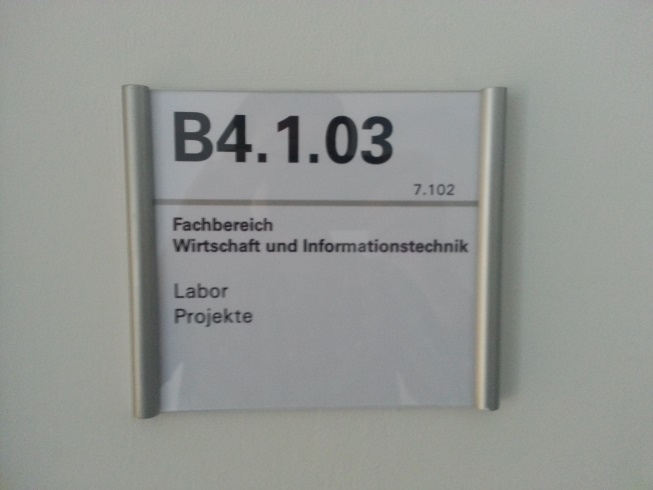
\includegraphics[width=\linewidth]{Bilder/Raumschild_gross}
\caption{Gesamtes Bild Raumschild}
\label{fig:RaumschildGross}
\end{figure}

\begin{figure}
\centering
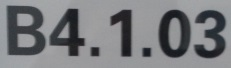
\includegraphics[width=\linewidth]{Bilder/Raumschild_klein}
\caption{Ausschnitt Raumschild}
\label{fig:RaumschildKlein}
\end{figure}

Damit die Raumschilder zuverl�ssig erkannt werden, ist es notwendig,
dass aufgenommene Bilder zun�chst auf den Bereich mit der Raumnummer
zugeschnitten werden. Dies erfordert einen hohen Entwicklungsaufwand.


\subsubsection{App Google Goggles}
Google
Goggles\footnote{\url{https://play.google.com/store/apps/details?id=com.google.android.apps.unveil}}
ist eine Android-App, die zur Erkennung von Text, Symbolen
und QR-Tags verwendet werden kann. Diese App lieferte in Tests auch bei
suboptimalen Bildern gute Ergebnisse. Au�erdem ist die App gut in das
Android-Umfeld eingebettet und l�sst sich leicht bedienen.

Allerdings gibt es f�r die Verwendung von Google Googles noch keine �ffentliche
API\footnote{\url{http://stackoverflow.com/questions/2080731/google-goggles-api}}.
Diese ist zwar von Google geplant, aber nie umgesetzt worden. Auch wenn die
App eine komfortable M�glichkeit zur OCR-Erkennung bietet, kann diese ohne
API nicht in unserem Projekt verwendet werden.


